\documentclass[12pt,a4paper,titlepage]{article}

\setlength{\parskip}{\baselineskip} % Increase space between paragraphs
\setlength{\parindent}{0pt} % No indentation at paragraph level
\renewcommand{\familydefault}{cmss}

\usepackage[ngerman]{babel} % This is needed for umlauts
\usepackage[utf8]{inputenc} % This is needed for umlauts
\usepackage[T1]{fontenc} % This is needed for correct output of umlauts in pdf
\usepackage[pdftex,breaklinks,colorlinks,
citecolor=blue,
urlcolor=blue,
linkcolor=blue]{hyperref}
\usepackage{graphicx}
\usepackage[german]{cleveref} % Prepend \ref with corresponding label
% Use smaller margins
\usepackage[cm]{fullpage}
\usepackage{titlepic}
\usepackage{float}
\usepackage{subfig}
\usepackage[german]{cleveref} % Prepend \ref with corresponding label

% 'graphicx' configuration
\graphicspath{ {img/} }
\DeclareGraphicsExtensions{.jpg}

% Copy title, author to PDF metadata
\makeatletter
\AtBeginDocument{
  \hypersetup{
    pdftitle = {\@title},
    pdfauthor = {\@author}
  }
}
\makeatother

\title{Scratch}
\author{Hr. Walter, Hr. Ehret und Hr. Ribeaud}
\titlepic{
\includegraphics[scale=0.5]{scratch_logo.jpg}}

\begin{document}

\maketitle

\tableofcontents
\clearpage

\section{Projekt 1: Formel 1}
\label{sec:projekt1}

Dieses Projekt ist ein Autosimulator. Die Bühne zeigt eine Rennstrecke, über die ein Auto fährt. Du steuerst das Auto mit den Pfeiltasten. Immer wenn du auf der rechten Pfeiltaste drückst, dreht es sich um ein Stückchen nach rechts. Wenn du auf der linken Pfeiltaste drückst, dreht es sich nach links. Das Auto fährt mit konstanter  Geschwindigkeit. Wenn es die Strasse verlässt, hält es an.

\subsection{Die Rennstrecke}
\label{sub:rennstrecke}

Lege ein neues Projekt an und speichere es in deinem Projektordner z.B. unter dem Name \textit{auto} ab. Als erstes zeichnest du die Rennstrecke.

Klicke auf das Symbol der Bühne und wähle den Reiter \textit{Hintergründe}. Klicke dann auf die Schaltfläche \textit{Bearbeiten}.

\begin{figure}[H]
\centering
\subfloat{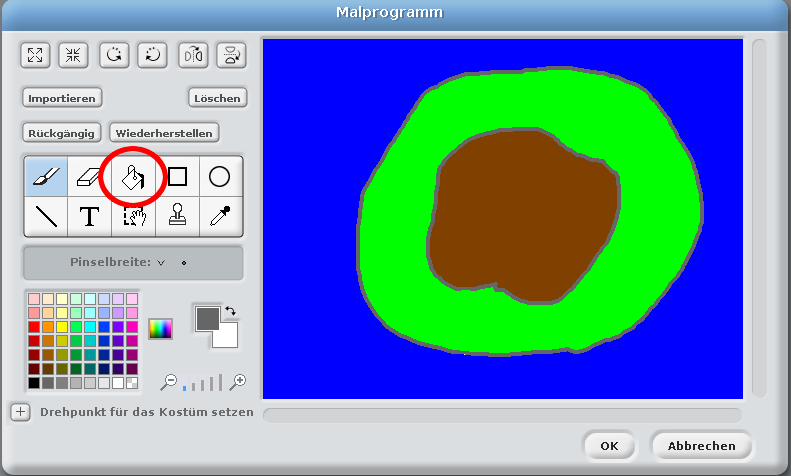
\includegraphics[width=.45\linewidth]{rennbahn1.png}}
\qquad
\subfloat{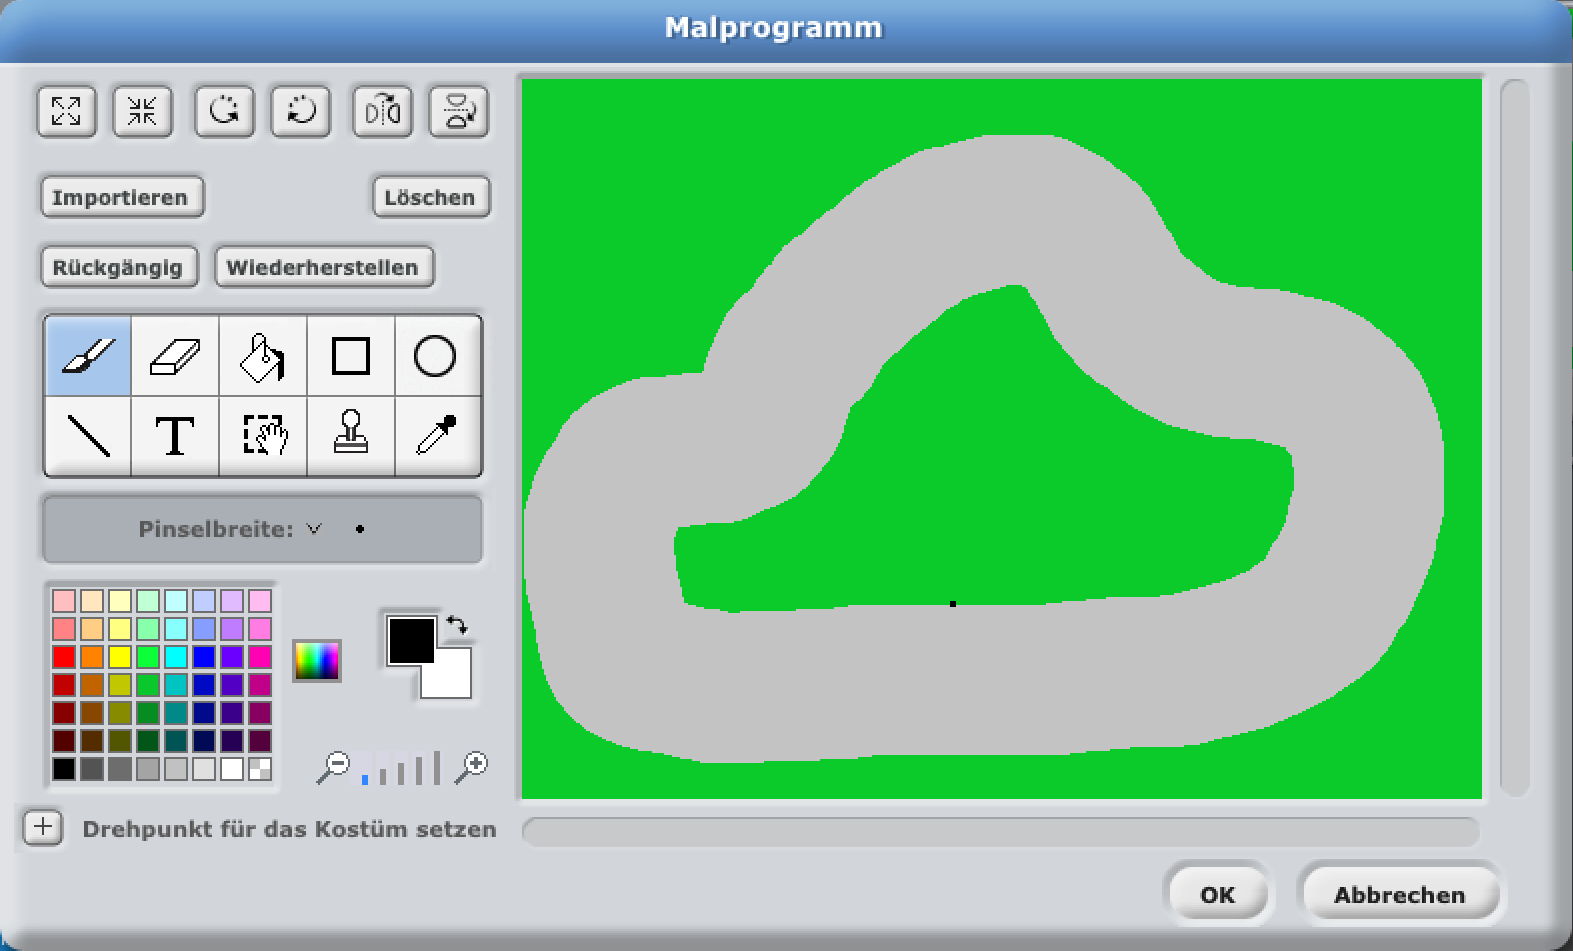
\includegraphics[width=.45\linewidth]{rennbahn2.png}}
\caption{Rennbahn als Bühnenbild}
\label{fig:rennbahn}
\end{figure}

\subsection{Das Auto}
\label{sub:auto}

Jedes neue Scratch-Projekt enthält bereits ein Objekt - die Katze. Aber jetzt brauchst du keine Katze, du brauchst ein Auto.

Das Malprogramm, um ein neues Sprite zu zeichnen, kann sich auf eine der folgenden Weisen öffnen:

\begin{itemize}
\item Doppelklicken auf der Katze, dann Schaltfläche \textit{Malen} neben \textit{Neues Kostüm:} anklicken.
\item Klicke dann auf die Schaltfläche \textit{Neues Objekt Malen} 
\includegraphics[height=\ht\strutbox]{neues_objekt.png}
\end{itemize}

Halte die Form klar und einfach. Denn das Auto wird auf dem Bildschirm nur zu sehen sein. Vergiss nicht, dem neuen Objekt einen sinnvollen Namen zu geben, z.B. \textbf{Auto}.

\begin{figure}[H]
\centering
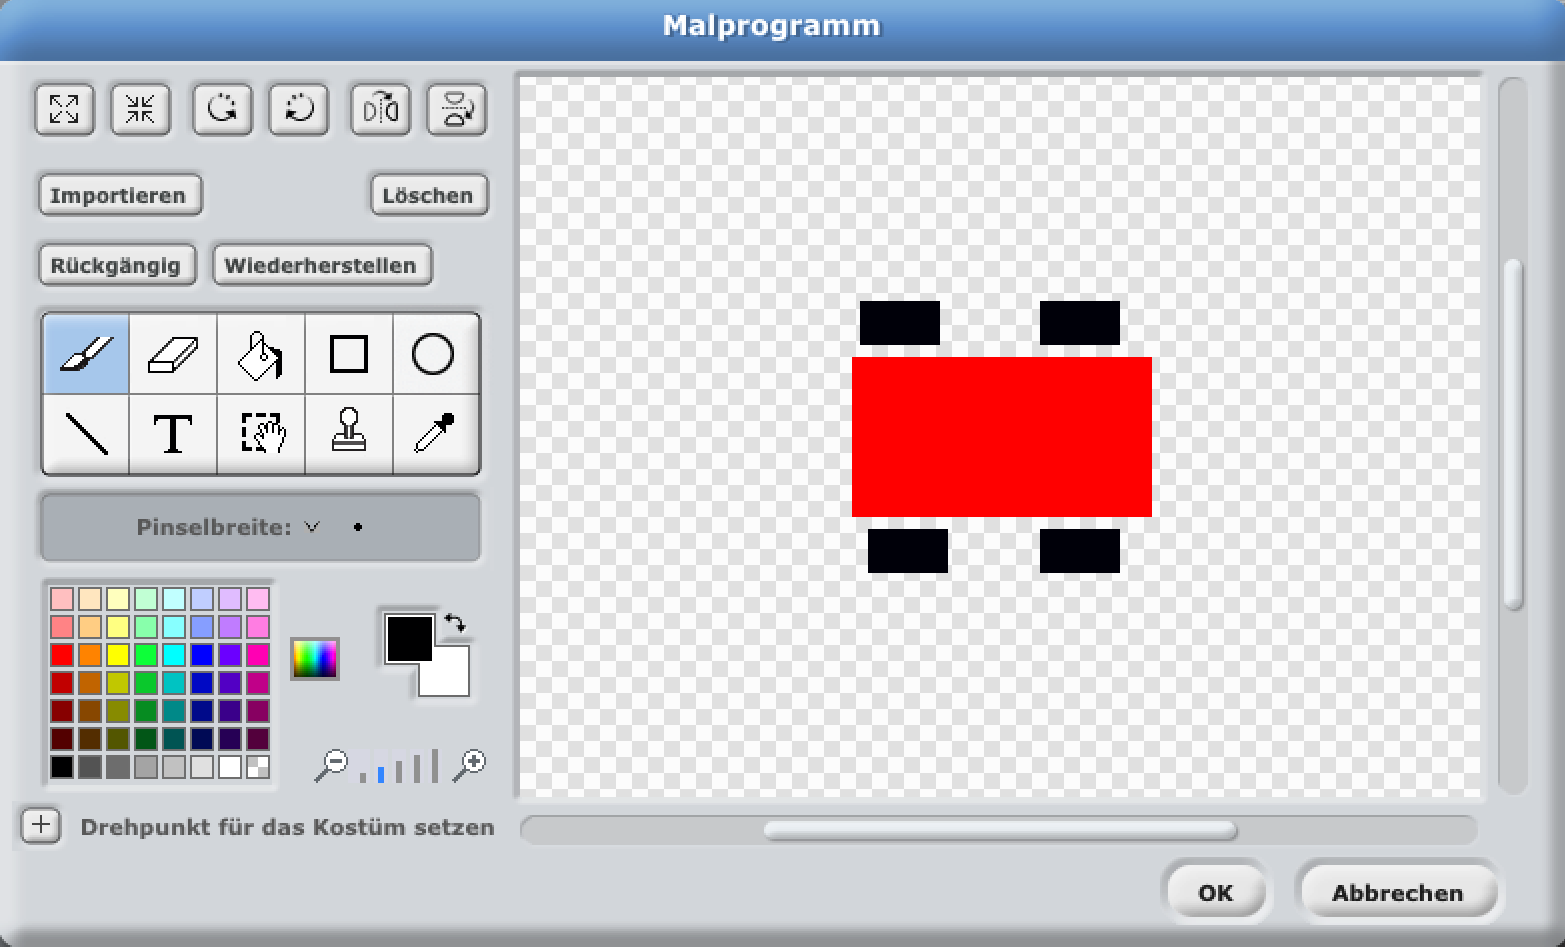
\includegraphics[scale=.3]{auto.png}
\caption{Ein Auto. Du kannst auch ein realisticheres Bild eines Formel-1-Wagens von oben zeichnen. Tipp: Zeichne zuerst ein rotes Rechteck und entferne dann mit dem Radiergummi kleinere Stücke.}
\label{fig:auto}
\end{figure}

\subsection{Die Skripte}
\label{sub:skripte}

Das Auto-Objekt erhält für die Steuerung \textbf{drei} Skripte. Das erste Skript wird zu Beginn einmal gestartet und läuft dann so lange, bis der Wagen von der Bahn abkommt und die grüne Umgebung berührt.

Die beiden anderen Skripte werden immer ausgeführt, und zwar immer dann, wenn eine Pfeiltaste gedrückt wird.

\subsection{Fragen zum Autorennen}

\begin{itemize}
\item Wie kannst du das Auto schneller machen? Es gibt zwei Möglichkeiten!
\item Was ändert sich, wenn in \textit{Zeige Richtung...}- Anweisung statt der Zahl 90 die Zahl 0 steht?
\end{itemize}

\subsection{Erweiterungen}

\begin{enumerate}
\item Lass einen Klang lauten, wenn das Auto die Strasse verlässt.
\item Das Auto sollte weiterfahren, wenn du die Leertaste drückst.
\item Anzeige einer Stoppuhr.
\end{enumerate}

\subsubsection{Gas geben und bremsen}

Wenn du in deinem Rennwagen Gas gibst, wird die Geschwindigkeit höher. Wenn du bremst, wird sie niedriger. Das heisst: Die Schrittlänge ändert sich. Das Problem ist also, die Zahl in dem \textit{Gehe}-Baustein. Wenn die Geschwindigkeit geändert werden kann, darf hier überhaupt keine feste Zahl stehen.

Was tun? Die Lösung ist eine \textbf{Variable}. An Stelle einer Zahl setzen wir in das Zahlfenster eine Variable, z.B. 
\includegraphics[height=\ht\strutbox]{speed.png} (engl. \textit{speed}=Geschwindigkeit).

\subsubsection{Autorennen mit mehreren Szenen}

Erweitere das Projekt auf folgende Weise. Die Rennstrecke erstreckt sich über \textit{zwei} Hintergrundbilder wie in \cref{fig:erweiterung} Wenn der Rennwagen den rechten Rand des ersten Bildes berührt, erscheint ein neues Hintergrundbild mit dem zweiten Teil der Rennstrecke. Der Wagen springt an den linken Rand der Bühne und fährt von links über das Bild weiter. Anders herum funktioniert es genauso: Wenn der Wagen sich im rechten Teil der Rennstrecke befindet und gegen den linken Rand fährt, ändert sich wieder das Hintergrundbild.

\begin{figure}[H]
\centering
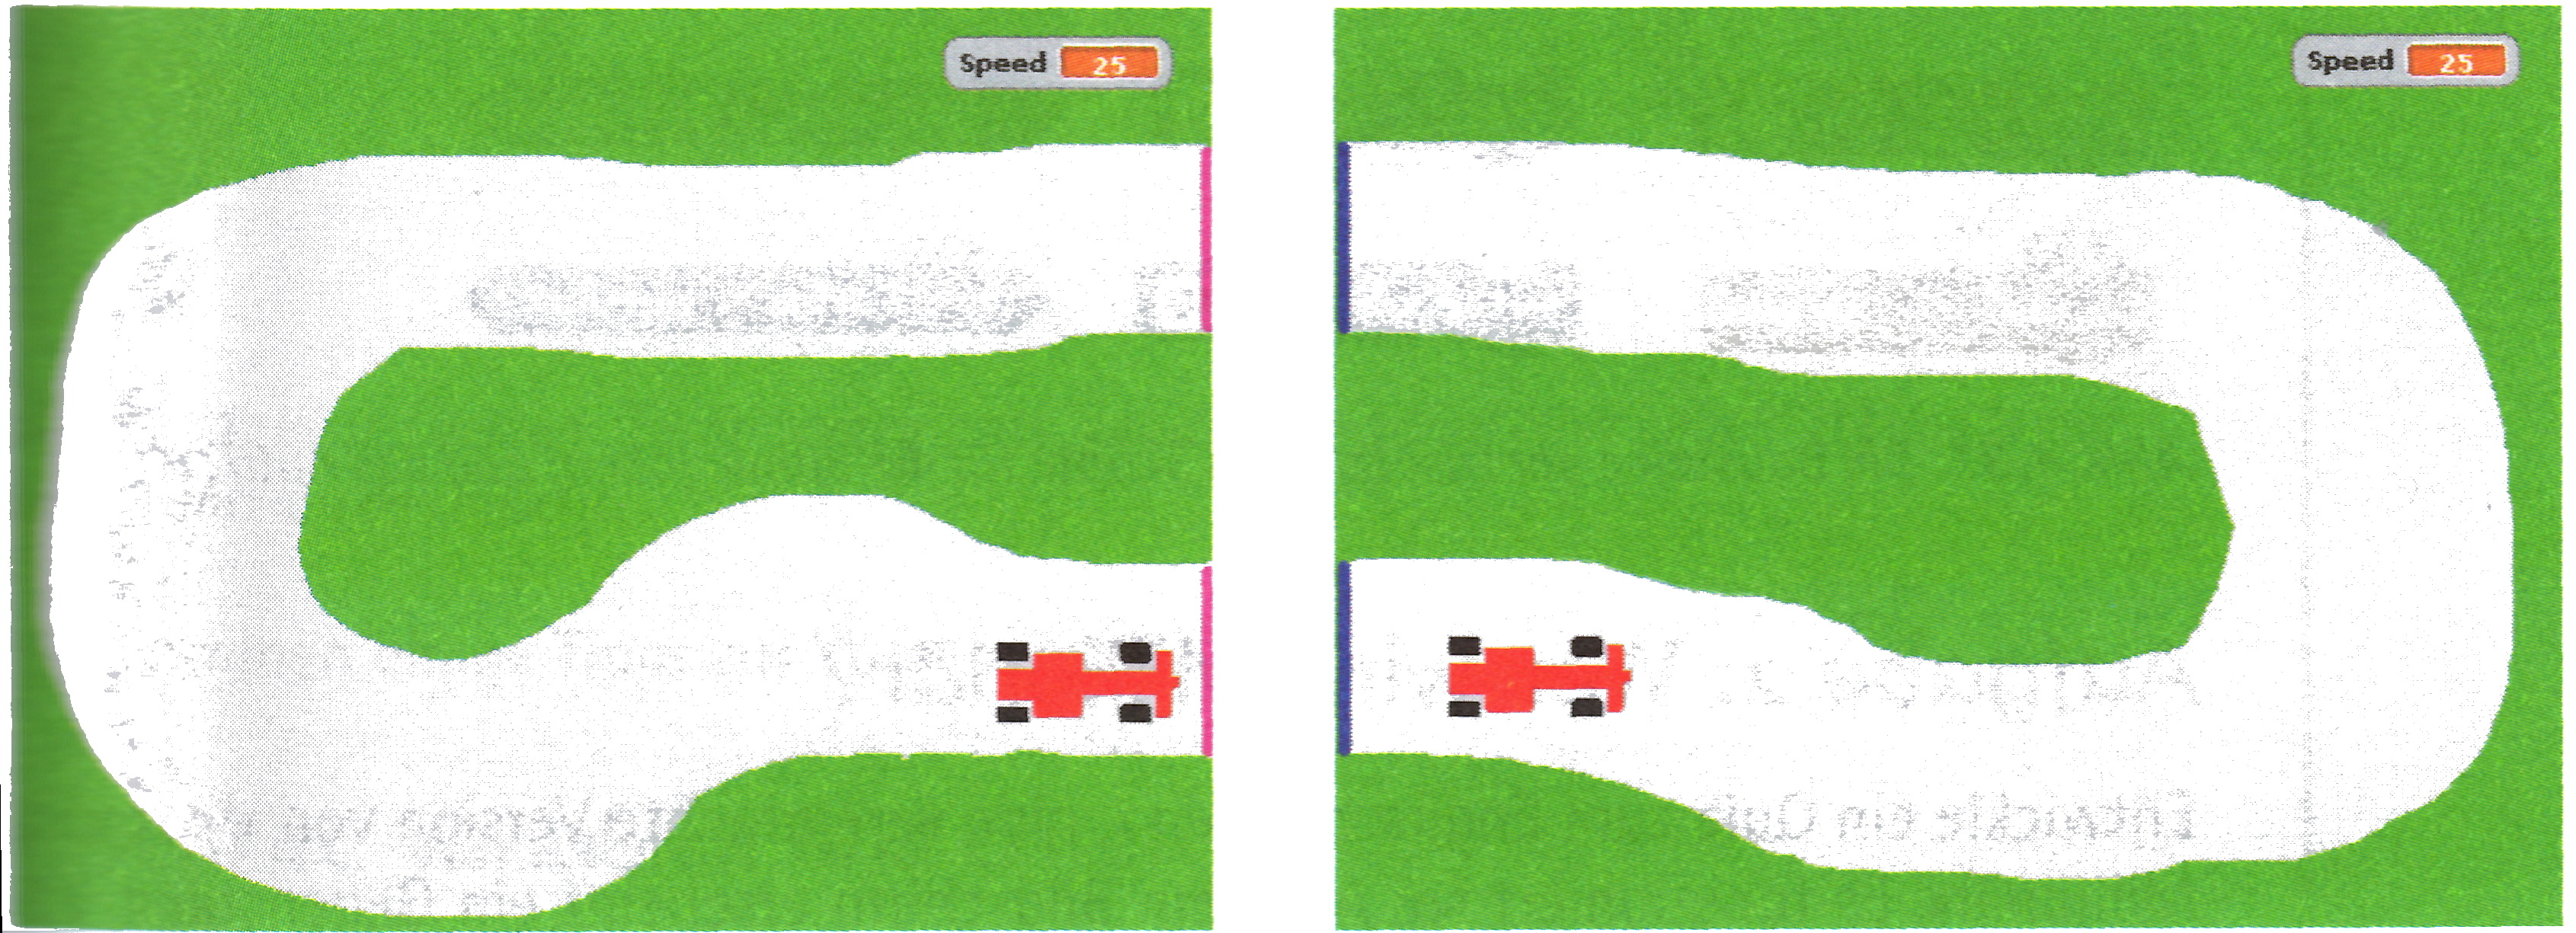
\includegraphics{rennbahn3.jpg}
\caption{Eine Rennstrecke, die sich über zwei Hintergrundbilder erstreckt.}
\label{fig:erweiterung}
\end{figure}

\section{Projekt 2:}
\label{sec:projekt2}

\end{document}